\section{Appendix A: Data Description and Additional Background}

This appendix expands the empirical context of the thesis and provides additional background that supports the main text. Since the body of the thesis focuses on argument and interpretation, the appendix collects descriptive material that would otherwise interrupt the flow of the central narrative.

\subsection{Descriptive role of the asset universe}

The choice of assets in the thesis is not arbitrary. Each instrument represents a distinct dimension of the conventional financial system against which Bitcoin can be compared.

\begin{itemize}
    \item The S\&P 500 is used as a broad proxy for U.S. equity-market risk and general investor sentiment.
    \item The NASDAQ Composite captures a more growth-oriented and technology-heavy market segment, making it especially interesting in relation to crypto assets.
    \item Gold and silver ETFs represent precious-metal exposure, a domain frequently associated with hedging, inflation narratives, and safe-haven debates.
    \item The U.S. dollar index proxy reflects macro-defensive positioning and global dollar strength.
    \item Ethereum is included as a crypto-native comparison asset in order to contrast same-ecosystem dependency with cross-market dependency.
\end{itemize}

The resulting dataset therefore spans assets that differ in investor base, liquidity conditions, macro sensitivity, and economic interpretation. This diversity helps the thesis avoid overly narrow conclusions.

\subsection{Visual overview of the dataset}

Figure~\ref{fig:eda_prices_appendix} presents normalized price paths for the asset universe. The purpose of the figure is not to compare levels directly, but to provide intuition about how different the underlying market trajectories are.

\begin{figure}[H]
    \centering
    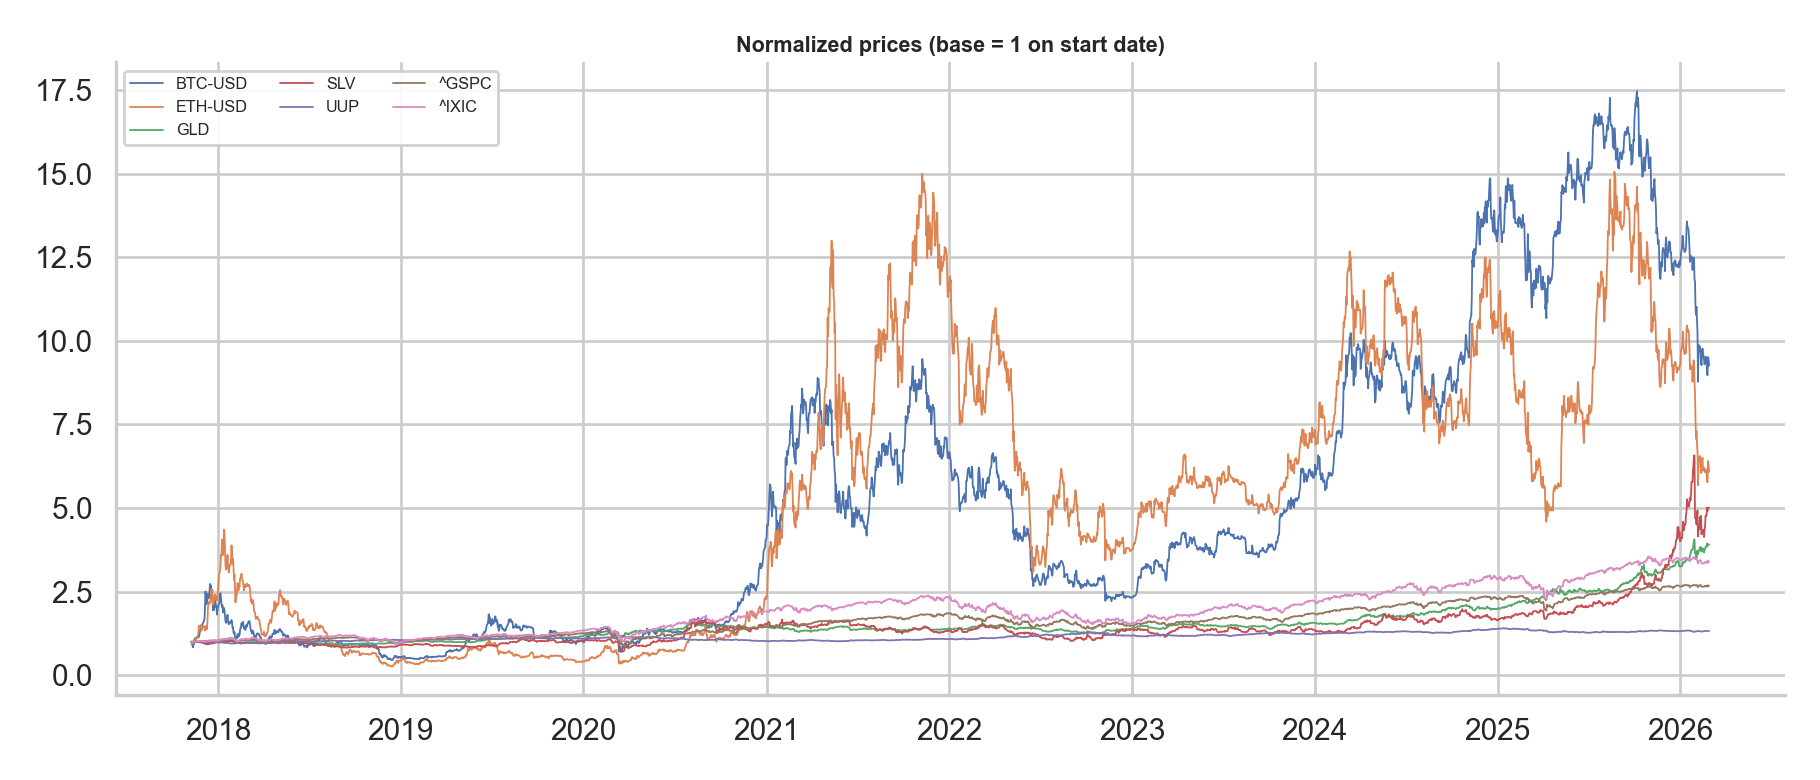
\includegraphics[width=0.95\textwidth]{../outputs/figures/eda_normalized_prices.png}
    \caption{Normalized prices of the assets included in the study.}
    \label{fig:eda_prices_appendix}
\end{figure}

Figure~\ref{fig:eda_vol_appendix} shows rolling volatility profiles. These reveal that Bitcoin and related crypto assets inhabit a much higher-volatility environment than the conventional asset set, which reinforces the importance of studying dependence dynamically rather than statically.

\begin{figure}[H]
    \centering
    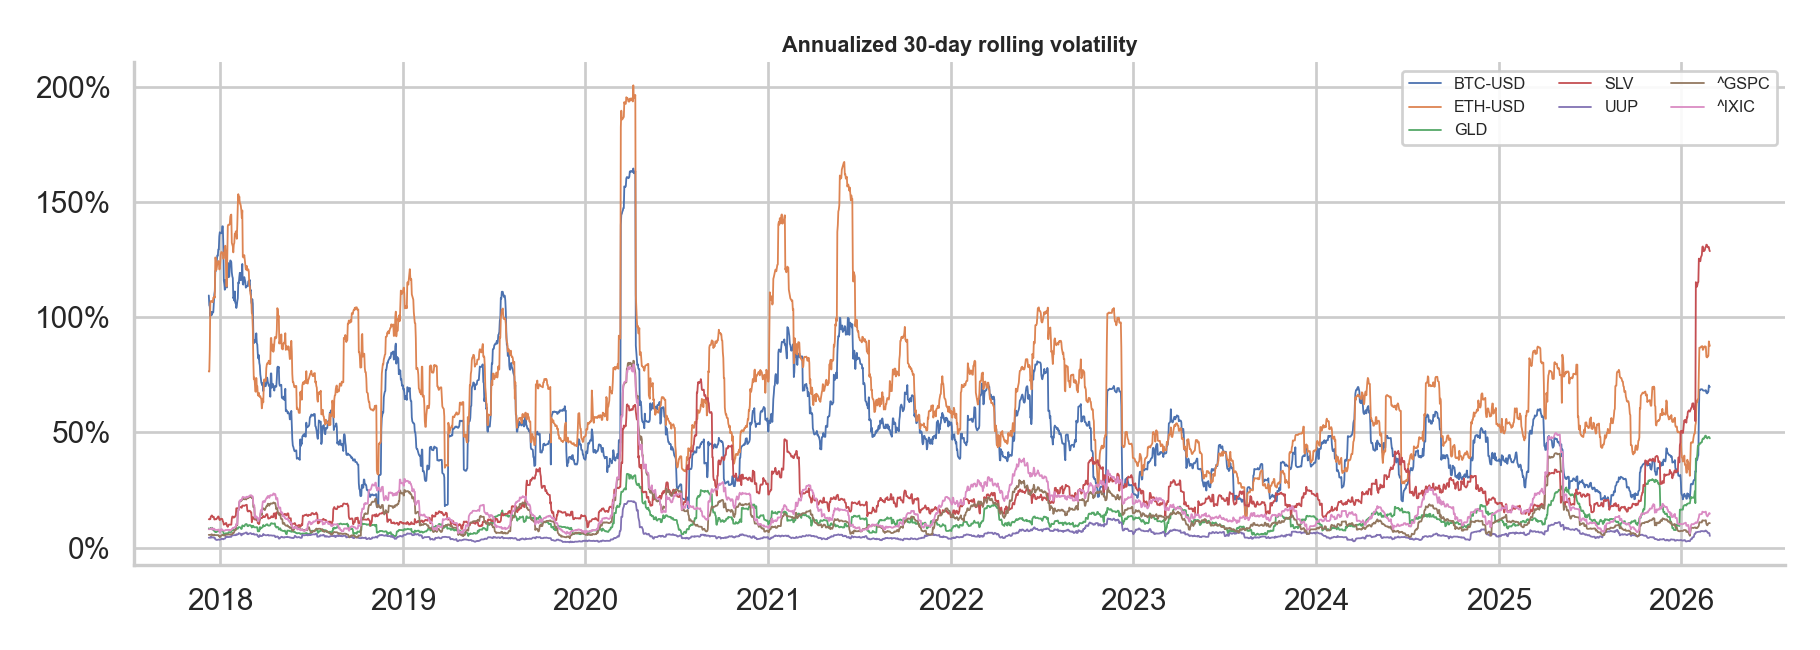
\includegraphics[width=0.95\textwidth]{../outputs/figures/eda_rolling_vol.png}
    \caption{Rolling volatility across the asset universe.}
    \label{fig:eda_vol_appendix}
\end{figure}

Figure~\ref{fig:eda_heatmap_appendix} provides the static correlation heatmap, while Figure~\ref{fig:eda_rollcorr_appendix} illustrates the dynamic rolling-correlation structure. Together, they motivate the main modeling choice of the thesis: static summaries are insufficient for describing the cross-market relations under study.

\begin{figure}[H]
    \centering
    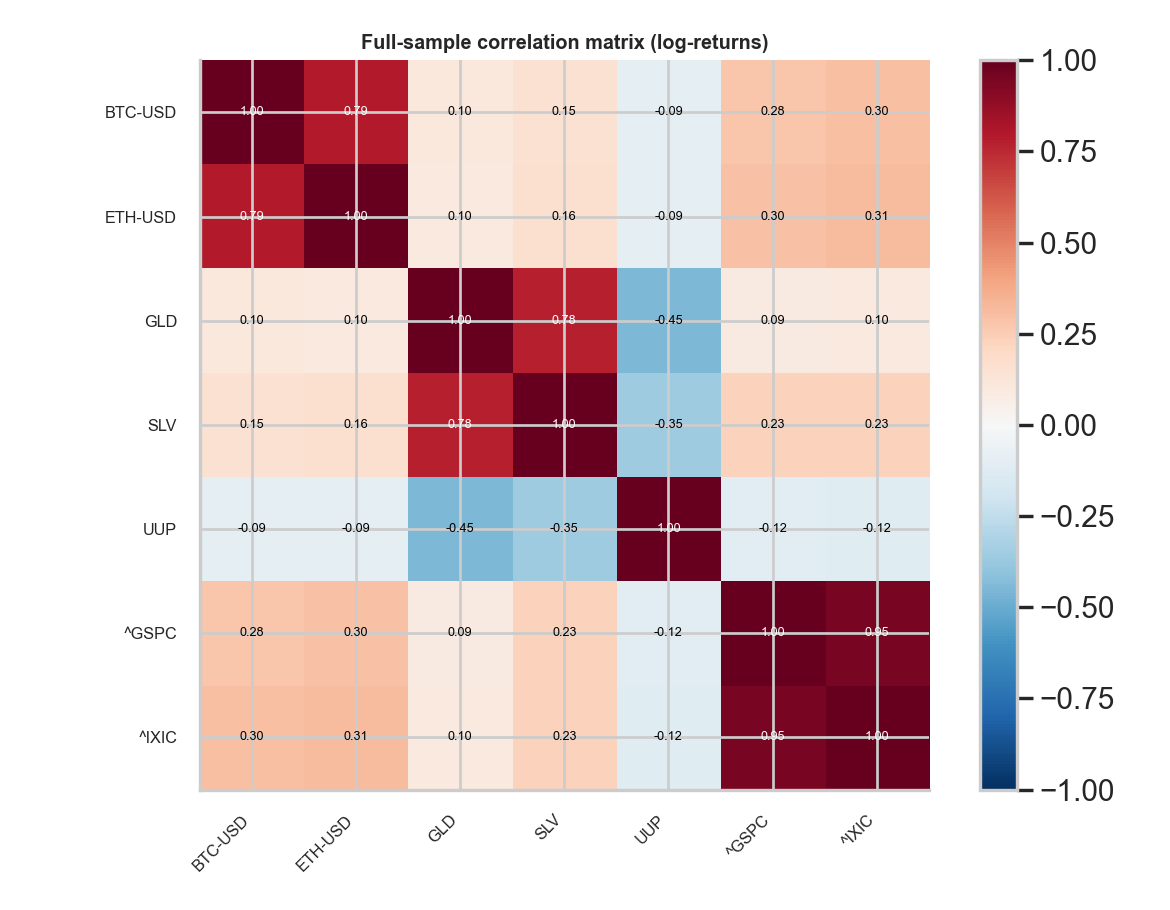
\includegraphics[width=0.85\textwidth]{../outputs/figures/eda_corr_heatmap.png}
    \caption{Static correlation heatmap of the return series.}
    \label{fig:eda_heatmap_appendix}
\end{figure}

\begin{figure}[H]
    \centering
    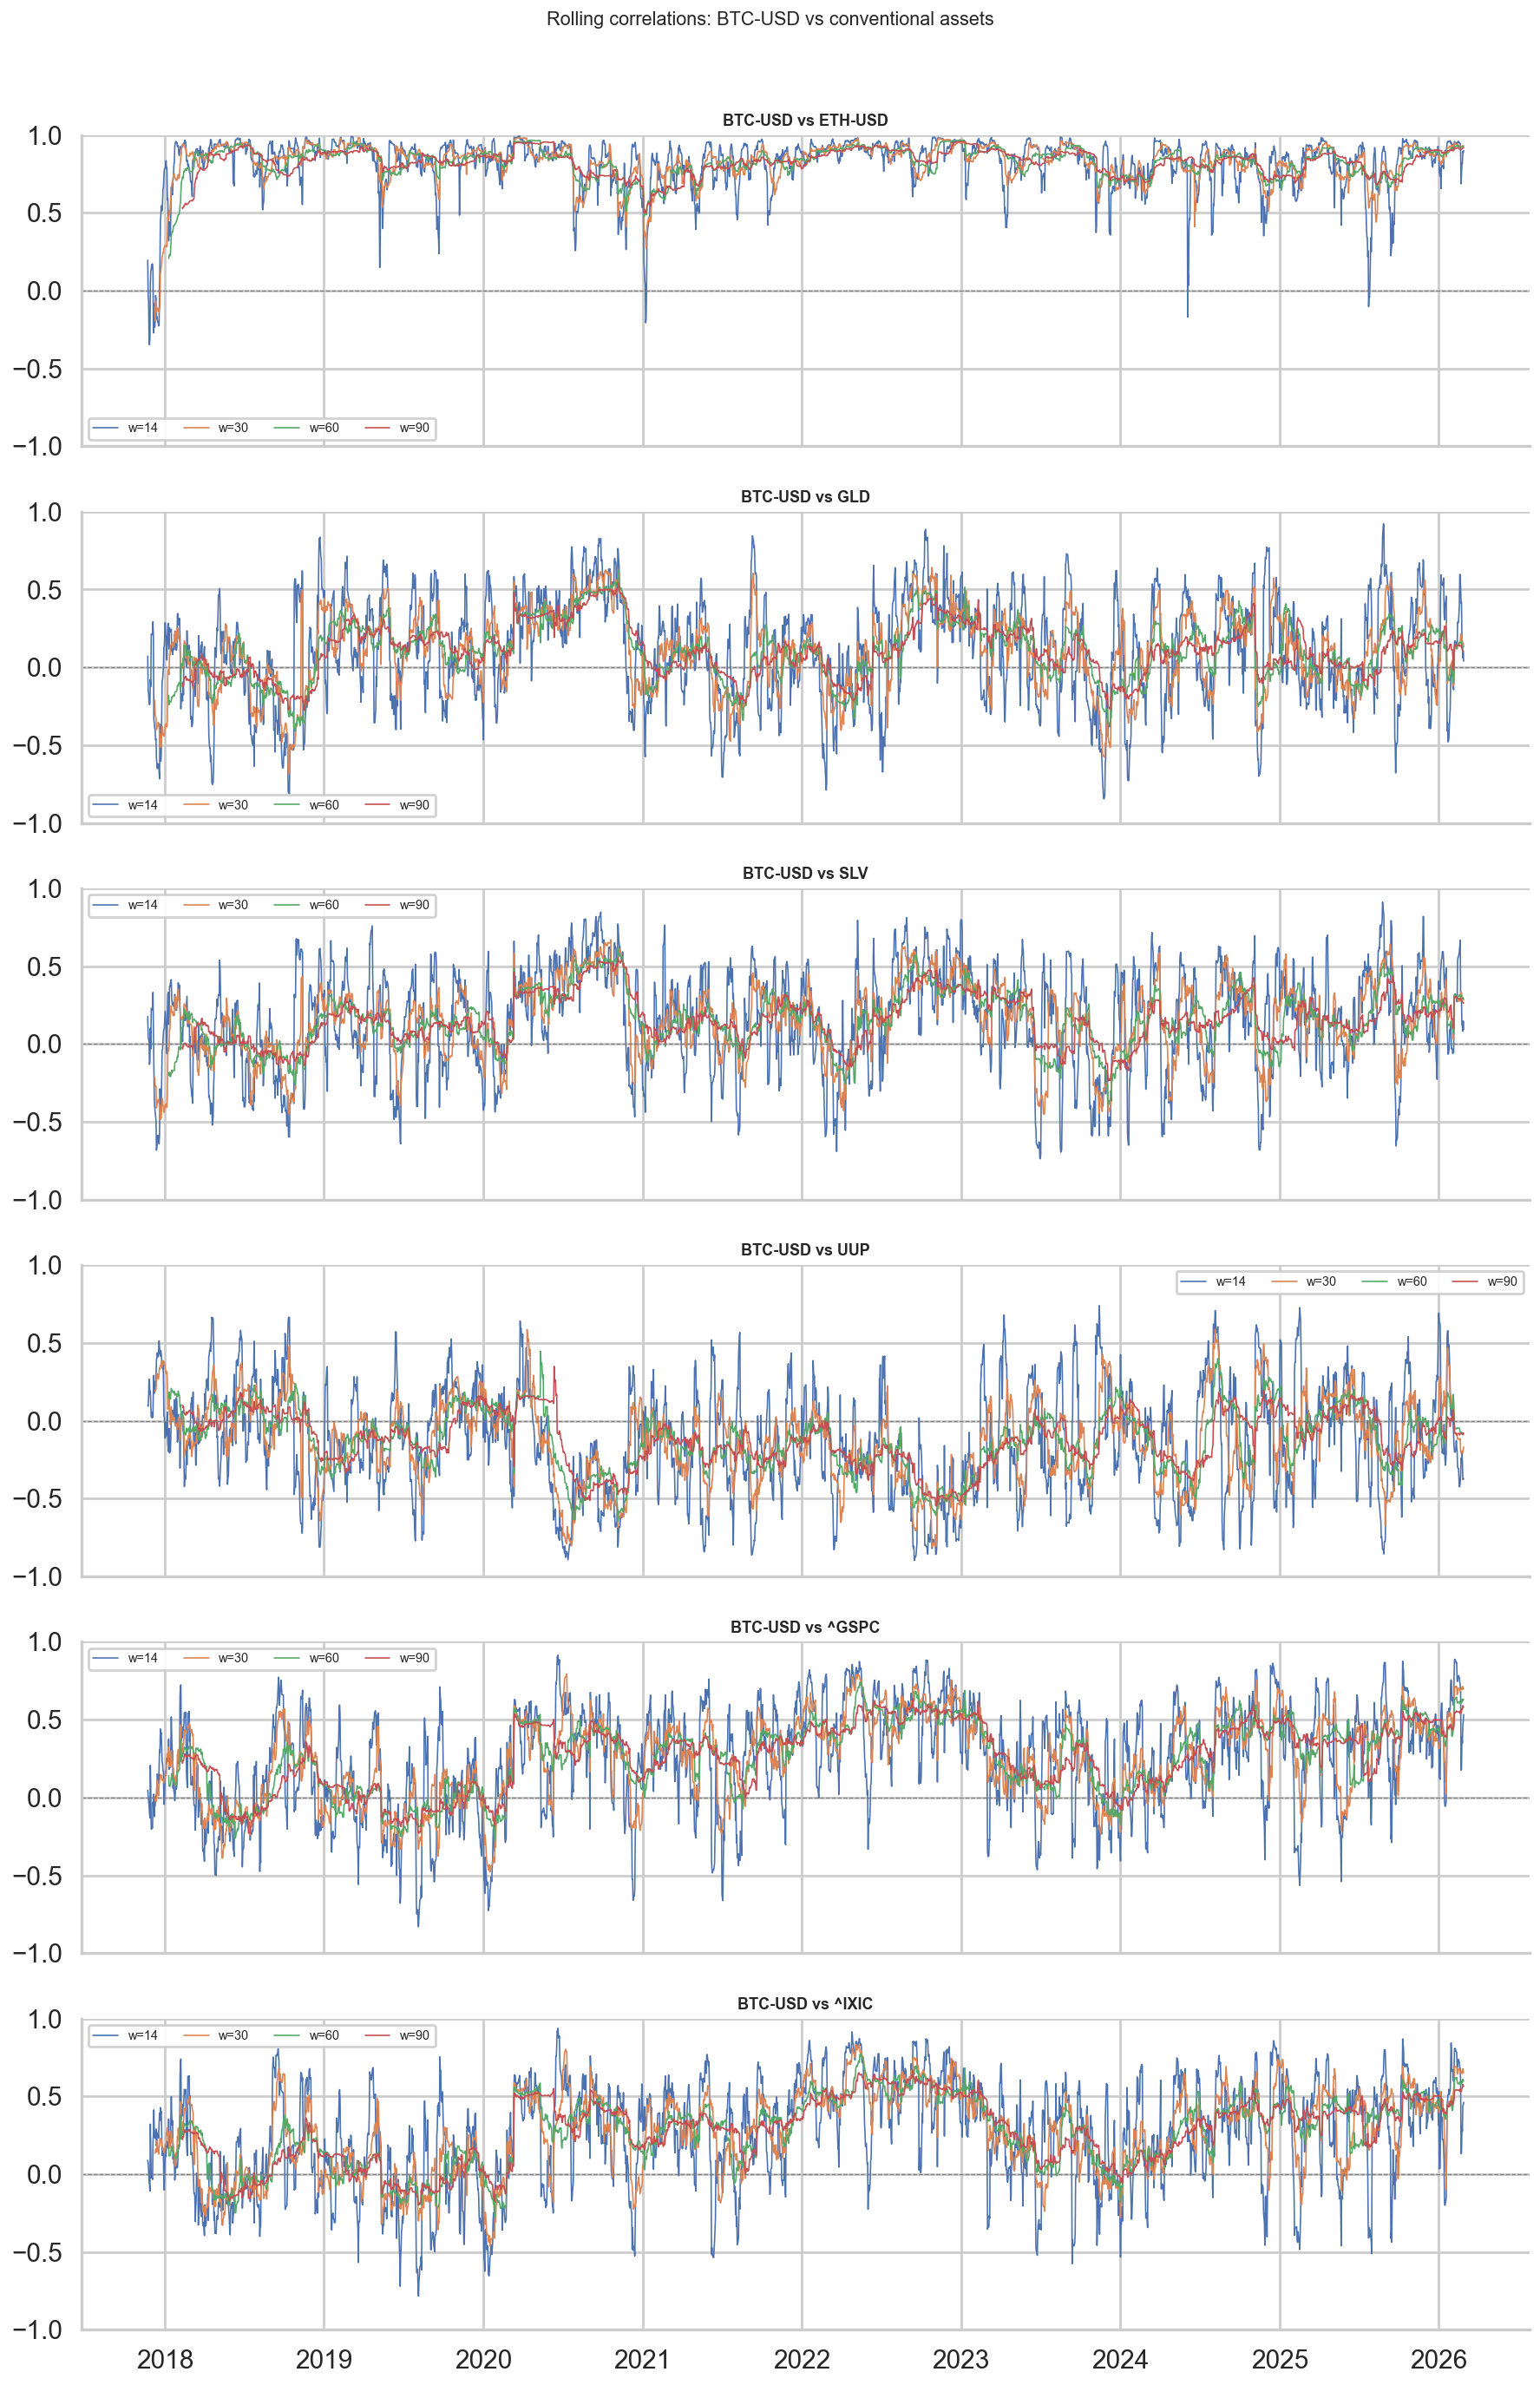
\includegraphics[width=0.98\textwidth]{../outputs/figures/eda_rolling_corr_all.png}
    \caption{Rolling correlation overview for the asset universe.}
    \label{fig:eda_rollcorr_appendix}
\end{figure}

\subsection{Why multiple rolling windows are used}

The thesis uses 14-day, 30-day, 60-day, and 90-day windows because no single dependence horizon is universally appropriate. A short window is more sensitive to recent shocks, but also noisier. A longer window produces a smoother target and often stronger persistence, but may react slowly to a regime shift. Evaluating several windows allows the empirical analysis to separate these effects.

The results indicate that the choice of window strongly shapes the forecastability profile. Longer windows are generally easier to forecast because they are smoother, but their predictive success is also more persistence-driven. Shorter windows react more quickly and are therefore more informative about local instability, although at the cost of noisier target behavior.

\subsection{Additional implementation remarks}

The project is organized so that each run of the pipeline produces consistent outputs in the \texttt{outputs/results}, \texttt{outputs/tables}, \texttt{outputs/figures}, and \texttt{outputs/predictions} directories. This structure is helpful not only for reproducibility but also for writing. Since the tables and figures are generated directly from the code pipeline, the gap between experiment execution and thesis writing is reduced.

Another useful implementation detail is that the notebook environment was aligned with the pipeline. Readability improvements were introduced in the notebooks so that figures are interpretable, benchmarks are selected robustly, and helper functions can be reused without fragile path assumptions. This matters because, in practice, exploratory notebooks often become a weak point in academic projects if they drift away from the main pipeline.

\subsection{Summary}

The appendix confirms an important methodological point: the empirical environment studied in this thesis is heterogeneous, nonstationary in economic interpretation, and rich enough to justify a time-varying dependency framework. The descriptive evidence supports the modeling strategy used in the main body of the thesis.
